% ============================ DAG DE AIRFLOW =========================
\section{Explicación del DAG de Airflow}
\label{sec:airflow}

La automatización se implementa en un único DAG, \texttt{github\_events\_pipeline}, definido en \repo{dags/github_events_dag.py}{dags/github\_events\_dag.py}. Contiene las seis etapas que exige el enunciado, encadenadas linealmente, y se ejecuta de forma programada cada hora.

\begin{figure}[H]
    \centering
    \begin{tikzpicture}[
        font=\scriptsize,
        task/.style={rectangle, draw=black, thick, rounded corners=2pt, minimum width=2.15cm, minimum height=1.25cm, align=center},
        arrow/.style={-{Stealth[scale=1.0]}, thick}
    ]
    \node[task, fill=gray!12] (t1) {\textbf{1}\\ \texttt{extract\_data}};
    \node[task, fill=gray!12, right=0.32cm of t1] (t2) {\textbf{2}\\ \texttt{validate\_}\\ \texttt{and\_clean}};
    \node[task, fill=green!16, right=0.32cm of t2] (t3) {\textbf{3}\\ \texttt{load\_mongodb}};
    \node[task, fill=blue!14, right=0.32cm of t3] (t4) {\textbf{4}\\ \texttt{transform\_load\_}\\ \texttt{cassandra}};
    \node[task, fill=violet!16, right=0.32cm of t4] (t5) {\textbf{5}\\ \texttt{build\_graph\_}\\ \texttt{neo4j}};
    \node[task, fill=orange!16, right=0.32cm of t5] (t6) {\textbf{6}\\ \texttt{generate\_kpis}};
    \draw[arrow] (t1) -- (t2); \draw[arrow] (t2) -- (t3); \draw[arrow] (t3) -- (t4);
    \draw[arrow] (t4) -- (t5); \draw[arrow] (t5) -- (t6);
    \end{tikzpicture}
    \caption{Tareas del DAG \texttt{github\_events\_pipeline} y su orden de ejecución.}
    \label{fig:dag}
\end{figure}

\subsection{Etapas}

Cada tarea es un \texttt{PythonOperator} que invoca una función del paquete \texttt{src/}. La lógica vive fuera del DAG para que los mismos módulos puedan ejecutarse desde la carga histórica y desde los \textit{notebooks}.

\begin{table}[H]
\centering
\caption{Etapas del DAG: qué lee y qué escribe cada una}
\label{tab:etapas}
\vspace{0.2cm}
\footnotesize
\begin{tabular}{@{}cp{3.3cm}p{4.9cm}p{5.4cm}@{}}
\toprule
\textbf{\#} & \textbf{Tarea} & \textbf{Lee} & \textbf{Escribe} \\
\midrule
1 & \texttt{extract\_data} &
Archivo horario de GH Archive (HTTP). &
\texttt{data/raw/AAAA-MM-DD-H.json.gz}. Si ya existe, no lo vuelve a descargar. \\
\addlinespace
2 & \texttt{validate\_and\_clean} &
Archivo crudo, línea a línea, sin cargarlo entero en memoria. &
Archivo intermedio JSONL con los eventos válidos, y estadísticas de calidad (crudos, válidos, duplicados, rechazados y motivos). \\
\addlinespace
3 & \texttt{load\_mongodb} &
Archivo intermedio. &
Colección \texttt{events} (\textit{upsert} por \texttt{\_id}) y un documento en \texttt{ingestion\_log}. \\
\addlinespace
4 & \texttt{transform\_load\_\bk{}cassandra} &
\textbf{MongoDB}: eventos de la hora, por el índice de \texttt{created\_at}. &
Cinco tablas de agregados de Cassandra y la fila de la hora en \texttt{pipeline\_runs}. \\
\addlinespace
5 & \texttt{build\_graph\_neo4j} &
\textbf{Cassandra}: partición de la hora en \texttt{user\_repo\_\bk{}interactions\_\bk{}by\_hour}. &
Nodos y relaciones en Neo4j (\texttt{MERGE}); marca \texttt{loaded\_neo4j} en \texttt{pipeline\_runs}. \\
\addlinespace
6 & \texttt{generate\_kpis} &
\textbf{Las tres bases}: Cassandra (KPI 1--3), MongoDB (KPI 4), Neo4j (KPI 5). &
Cinco filas en \texttt{kpis\_by\_date} para el día de la hora procesada. \\
\bottomrule
\end{tabular}
\end{table}

Las tareas se comunican por XCom, pero \textbf{solo intercambian metadatos}: el nombre y la ruta del archivo, la hora procesada y las estadísticas de cada etapa. Los eventos nunca viajan por XCom; cada etapa los lee de la capa de almacenamiento anterior. Esto mantiene pequeña la base de metadatos de Airflow y hace que cada etapa sea reejecutable de forma independiente.

\subsection{Programación}

\begin{table}[H]
\centering
\caption{Parámetros de programación y tolerancia a fallos del DAG}
\label{tab:dag-params}
\vspace{0.2cm}
\small
\begin{tabular}{@{}llp{7.6cm}@{}}
\toprule
\textbf{Parámetro} & \textbf{Valor} & \textbf{Efecto} \\
\midrule
\texttt{schedule}           & \texttt{@hourly}  & Una corrida al inicio de cada hora. \\
\texttt{catchup}            & \texttt{False}    & No repone corridas pasadas al activar el DAG; el pasado se carga con el \textit{script} de carga histórica. \\
\texttt{max\_active\_runs}  & 1                 & Nunca hay dos corridas simultáneas, lo que protege las tablas diarias de Cassandra, que se actualizan leyendo y reescribiendo. \\
\texttt{retries}            & 3                 & Reintentos automáticos por tarea. \\
\texttt{retry\_delay}       & 5 minutos         & Espera entre reintentos; cubre el caso de que el archivo de la hora aún no esté publicado. \\
Ejecutor                    & \texttt{LocalExecutor} & Las tareas corren como procesos del planificador. \\
\bottomrule
\end{tabular}
\end{table}

Cada corrida procesa la hora \texttt{data\_interval\_start} $-$ 2\,h. El retraso de dos horas absorbe la demora con la que GH Archive publica cada archivo; así, la corrida programada a las 05:00 UTC procesa el archivo de las 02:00 UTC.

\subsection{Idempotencia}

Un flujo programado debe poder reintentarse sin alterar el resultado. Cada etapa lo garantiza con el mecanismo propio de su base de datos:

\begin{itemize}[leftmargin=*]
    \item \textbf{Extracción:} descarga a un archivo temporal y lo renombra al terminar; si el destino ya existe, no descarga.
    \item \textbf{MongoDB:} \textit{upsert} con \texttt{\$setOnInsert} sobre el \texttt{\_id} del evento.
    \item \textbf{Cassandra:} la etapa se omite si la hora ya figura en \texttt{pipeline\_runs}.
    \item \textbf{Neo4j:} la etapa se omite si \texttt{pipeline\_runs.loaded\_neo4j} es mayor que cero para esa hora.
    \item \textbf{Indicadores:} se recalculan completos y se sobrescriben por clave primaria (día, indicador).
\end{itemize}

\subsection{Evidencia de Ejecución}

\begin{figure}[H]
    \centering
    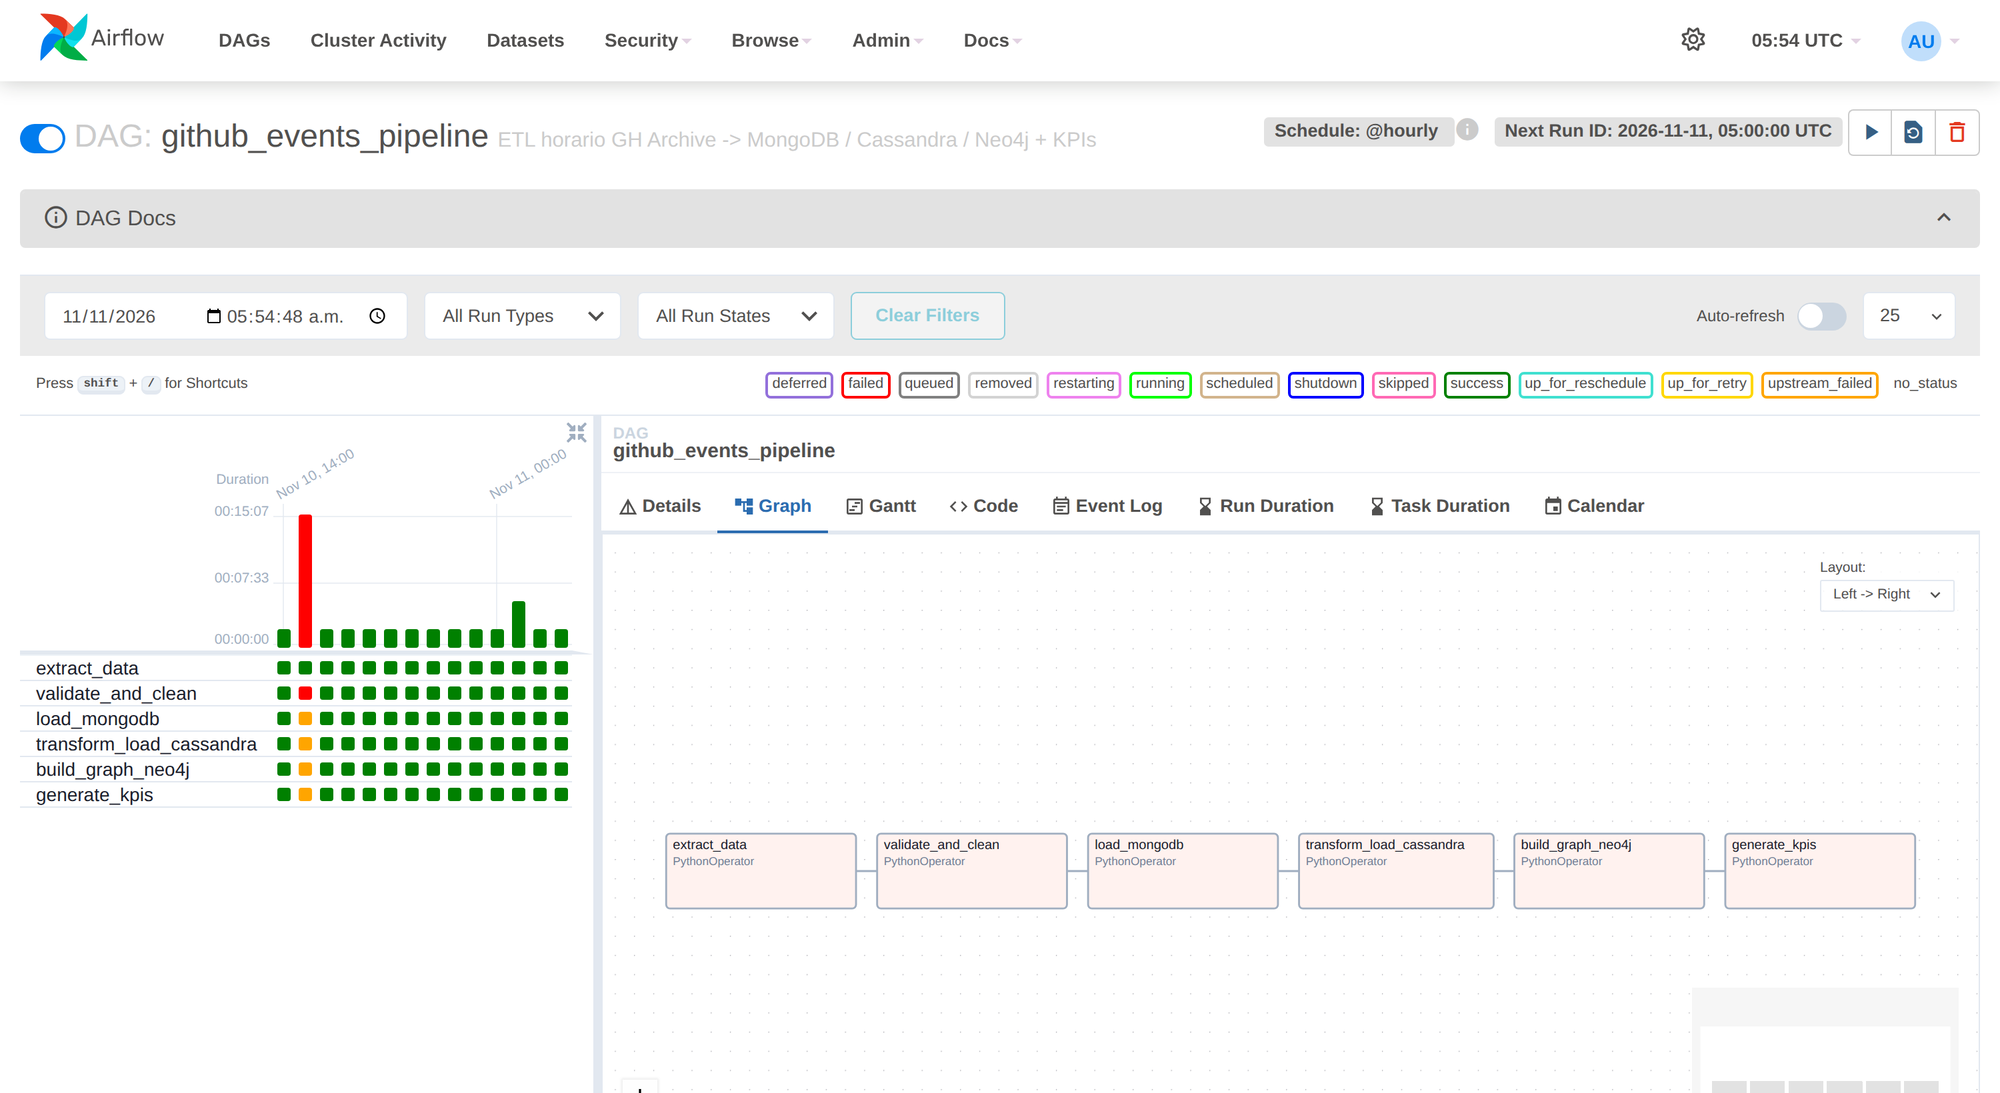
\includegraphics[width=\textwidth]{airflow-grafo.png}
    \caption{Interfaz de Airflow: DAG activo con programación \texttt{@hourly}. A la izquierda, el historial de corridas por tarea; a la derecha, el grafo de las seis tareas.}
    \label{fig:airflow-grafo}
\end{figure}

Desde su activación, el 10 de noviembre de 2026 a las 14:36 UTC, hasta la captura de la Figura~\ref{fig:airflow-grafo}, el DAG registró 14 corridas: 13 exitosas y 1 fallida. Una corrida normal sobre una hora de noviembre (unos 3,500 eventos) completa las seis etapas en un tiempo de entre 7 y 21 segundos.

\subsection{Diagnóstico de la Corrida Fallida}
\label{subsec:fallo}

La corrida programada para las 14:00 UTC del 10 de noviembre falló en la tarea \texttt{validate\_and\_clean} tras agotar sus tres intentos (15:00, 15:05 y 15:10 UTC). El registro de la tarea muestra el mismo error en los tres:

\begin{lstlisting}[style=plano]
PermissionError: [Errno 13] Permission denied:
    '/opt/airflow/data/processed/2026-11-10-12.clean.jsonl'
\end{lstlisting}

\paragraph{Causa.} El error no tiene relación con los datos. La carpeta \texttt{data/} está montada a la vez en el contenedor de Airflow, cuyos procesos corren con el identificador de usuario 50000, y en el de Jupyter, que usa el 1000. La hora 12 de ese día ya había sido procesada por la carga histórica lanzada desde Jupyter, que reescribió el archivo intermedio a las 14:44 UTC, dieciséis minutos antes de la corrida; el archivo existía y pertenecía al usuario 1000. Al intentar abrirlo para sobrescribirlo, Airflow no tenía permiso de escritura sobre él. El listado de la carpeta lo confirma: los archivos de las horas 10 y 12 pertenecen al usuario 1000, y los de las horas 11 y 13, al 50000.

\paragraph{Impacto.} Ninguno sobre los datos: la hora 12 figura en \texttt{pipeline\_runs} con sus 3,778 eventos, registrada a las 14:36 UTC, antes de la corrida fallida, que por tanto habría sido redundante.

\paragraph{Corrección.} La escritura del archivo intermedio se cambió a una \textbf{escritura atómica}: se escribe en un archivo temporal propio del proceso y se reemplaza el destino con \texttt{os.replace}. Reemplazar una entrada de directorio solo requiere permiso sobre la carpeta, no sobre el archivo previo, por lo que el conflicto desaparece; además, un proceso interrumpido ya no puede dejar un archivo intermedio a medio escribir.

\paragraph{Una segunda observación.} En \texttt{pipeline\_runs} faltan dos horas consecutivas: las 23:00 UTC del 10 de noviembre y las 00:00 UTC del 11. Corresponden a las corridas de las 01:00 y 02:00 UTC del día 11, que nunca se crearon porque el planificador no estuvo activo en ese intervalo (la corrida de las 00:00 UTC comenzó recién a las 04:49 UTC). Con \texttt{catchup=False} Airflow no repone esas corridas al reanudar. No es una pérdida de datos, puesto que los archivos siguen publicados en la fuente y el \textit{script} de carga histórica los incorpora, pero ilustra el costo de esa configuración: la continuidad depende de que el planificador no se detenga. El \textit{dashboard} hace visible la brecha al marcar el 10 de noviembre como día parcial, con 23 de 24 horas.
